\chapter{A-A WEAPONS}
\thumbtab{A-A}{5}
\localtableofcontents
\cleardoublepage

\section{AIR-TO-AIR GUNNERY}

\subsection{M-61 CANNON}

\begin{tcoloritemize}
    \blueitem{M-61}{
    Internally mounted, high fire-rate, 20mm rotary cannon

    \begin{subitemize}
        \item \textbf{Fire Rate} --- 6000rpm
        \item \textbf{Round Size} --- 20mm
        \item \textbf{Ammo Capacity} --- 510 rounds
    \end{subitemize}}
\end{tcoloritemize}

\begin{figure}[htbp]
    \centering
    \fbox{
    \begin{minipage}[t][75mm][t]{100mm}
        \center{\large\textbf{M-61 OVERVIEW}}
        \begin{itemize}
            \item Some kind of overview figure
            \item maybe showing side on profile of the weapon?
        \end{itemize}
    \end{minipage}
    }
    \caption{M-61 Cannon}
\end{figure}
    
\begin{tcoloritemize}
    \blueitem{Ammunition Types}{
    \begin{subitemize}
        \item \textbf{HEI} --- \textbf{H}igh \textbf{E}xplosive \textbf{I}ncendiary
        \item \textbf{HEI-T} --- \textbf{H}igh \textbf{E}xplosive \textbf{I}ncendiary-\textbf{T}racer
        \item \textbf{AP} --- \textbf{A}rmor \textbf{P}iercing
        \item \textbf{TP} --- \textbf{T}arget \textbf{P}ractice
        \item \textbf{SAPHEI} --- \textbf{S}emi \textbf{A}rmor \textbf{P}iercing \textbf{H}igh \textbf{E}xplosive \textbf{I}ncendiary
    \end{subitemize}}
    \blueitem{Select GUN}{
    Via Dogfight --- AIM-9 \& GUN automatically selected

    \begin{subenumerate}
        \item \textbf{DGFT/MSL OVRD} \dotfill \textbf{DGFT}
    \end{subenumerate}
    
    Via MFD

    \begin{subenumerate}
        \item \textbf{Master Mode} \dotfill \textbf{A-A}
        \item \textbf{SMS OSB 1} \dotfill \textbf{Cycle to GUN}
    \end{subenumerate}}
\end{tcoloritemize}

\subsubsection{SMS CONTROLS}

\begin{tcoloritemize}
    \blueitem{Operating Mode}{}
    \blueitem{Sub-Mode}{}
    \blueitem{Selected Round}{}
\end{tcoloritemize}

\begin{figure}[htbp]
    \centering
    \fbox{
    \begin{minipage}[t][75mm][t]{100mm}
        \center{\large\textbf{MFD --- SMS --- GUN CONTROLS}}
        \begin{itemize}
            \item show sms gun page
            \item label each of the relevant controls explained in text
        \end{itemize}
    \end{minipage}
    }
    \caption{MFD SMS Gun Controls}
\end{figure}

\subsubsection{EEGS SYMBOLOGY}

\begin{tcoloritemize}
    \blueitem{EEGS}{\textbf{E}nhanced \textbf{E}nvelope \textbf{G}un\textbf{S}ight
    \begin{subitemize}
        \item \textbf{Provides multiple levels of symbology depending on presence of radar lock}
    \end{subitemize}}
    \blueitem{Level I}{Backup mode displaying only boresight cross in event of INS failure}
    \blueitem{Level II}{Operating mode prior to radar lock

    \begin{subitemize}
        \item \textbf{Boresight Cross} --- shows where gun / aircraft is pointed
        \item \textbf{EEGS Funnel}
        \begin{itemize}
            \item displays path of rounds through space
            \item funnel is of set width to judge distance --- adjust width to target wingspan, stabilize edges of funnel on wingtips and fire
        \end{itemize}
        \item \textbf{MGRS} --- \textbf{M}ultiple \textbf{R}eference \textbf{G}un\textbf{S}ight
        \begin{itemize}
            \item 5 line-segments pointing towards boresight
            \item reference for high aspect snap shots (placeing target on MGRS line should have it fly through gun cross)
        \end{itemize}
    \end{subitemize}
    
    Reference symbology in \cref{fig:aaweap:m61:eegslvl2} and \cref{fig:aaweap:m61:funnelpipper}
    }
    \blueitem{Level III / IV}{Intermediate modes during radar lock acquisition}
    \blueitem{Level V}{Operating mode with radar lock. Level II symbology is retained with additional elements
    
    \begin{subitemize}
        \item \textbf{Level V Pipper}
        \begin{itemize}
            \item gunfire solution --- stabilize pipper on target and fire
            \item contains additional range/aspect cues
        \end{itemize}
        \item \textbf{Range Caret}
        \begin{itemize}
            \item displayed on \underline{inside} edge of level V pipper
            \item unwinds from 12 o'clock at 12'000ft counter-clockwise
        \end{itemize}
        \item \textbf{Aspect Caret} 
        \begin{itemize}
            \item displayed on \underline{outside} edge of level V pipper
        \end{itemize}
        \item \textbf{T-Symbol}
        \begin{itemize}
            \item \textbf{``--- + ---'' 1G Pipper} --- lead angle for non-maneuvering target,
            flanking horizontal lines indicate out-of-plane maneuver potential of target
            \item \textbf{``---'' Max-G Pipper} --- lead angle for target pulling max-G towards you
        \end{itemize}
        \item \textbf{BATR} --- \textbf{B}ullets \textbf{A}t \textbf{T}arget \textbf{R}ange
        \begin{itemize}
            \item displayed once rounds have been fired
            \item dissappears after last round has passed beyond target range
            \item useful to evaluate shots (also for training)
        \end{itemize}
    \end{subitemize}
    
    Reference symbology in \cref{fig:aaweap:m61:eegslvl5} and \cref{fig:aaweap:m61:funnelpipper}
    }
\end{tcoloritemize}

\begin{figure}[htbp]
    \centering
    \fbox{
    \begin{minipage}[t][75mm][t]{100mm}
        \center{\large\textbf{HUD --- EEGS LVL II}}
        \begin{itemize}
            \item show EEGS LVL II symbology of the HUD
            \item maybe with a simiplified target outline ``mid pull'' in the funnel?
            \begin{itemize}
                \item if don't have target here maybe put in marginfig below? (just show funnel with target at correct point to shoot)
                \item alternatively, maybe have separate figure just showing target in funnel here? (could be reused as marginfig below)
            \end{itemize}
        \end{itemize}
    \end{minipage}
    }
    \caption{EEGS LVL II HUD Symbology}
    \label{fig:aaweap:m61:eegslvl2}
\end{figure}

\begin{figure}[htbp]
    \centering
    \fbox{
    \begin{minipage}[t][75mm][t]{100mm}
        \center{\large\textbf{HUD --- EEGS LVL V}}
        \begin{itemize}
            \item show EEGS LVL V symbology of the HUD
            \item maybe with a simiplified target outline ``mid pull'' in the funnel?
            \begin{itemize}
                \item more necessary here since lvl V relies on having a lock
                \item maybe have separate figure just showing lvl 5 target pipper since there is a lot going on (could be reuses as marginfig below)
            \end{itemize}
        \end{itemize}
    \end{minipage}
    }
    \caption{EEGS LVL V HUD Symbology}
    \label{fig:aaweap:m61:eegslvl5}
\end{figure}

\begin{figure}[htbp]
    \centering
    \fbox{
    \begin{minipage}[t][50mm][t]{100mm}
        \center{\large\textbf{EEGS Funnel \& LVL V Pipper}}
        \begin{itemize}
            \item show both funnel and pipper as subfigs
            \item include target outline in firing position
            \item clearly mark level 5 pipper symbology elements
            \begin{itemize}
                \item batr
                \item range cue
                \item aspect
            \end{itemize}
        \end{itemize}
    \end{minipage}
    }
    \caption{EEGS Funnel \& Level V Pipper}
    \label{fig:aaweap:m61:funnelpipper}
\end{figure}

\marginfigeometry

\subsubsection{GUN SELECTION}
\begin{checklistenumerate}
    \blueitem{Select Gun}{
    \begin{subenumerate}
        \item \textbf{DGFT/Missile OVRD} \dotfill \textbf{DGFT}
    \end{subenumerate}

    or via SMS page

    \begin{subenumerate}
        \item \textbf{Master Mode} \dotfill \textbf{A-A}
        \item \textbf{SMS OSB 1} \dotfill \textbf{Cycle to GUN}
    \end{subenumerate}}
    \blueitem{EEGS Symbology}{Verify
    \begin{subitemize}
        \item \textbf{EEGS Level II} appears if no lock present
        \item \textbf{EEGS Level V} appears if target locked
    \end{subitemize}}
\end{checklistenumerate}

\subsubsection{EEGS LVL II EMPLOYMENT --- NO RADAR}
\begin{checklistenumerate}
    \blueitem{Prerequisites}{
    \begin{subitemize}
        \item \textbf{RF Switch} \dotfill \textbf{SILENT} \\
        \hfill (if desired, completely silences radar)
        \item \textbf{Selected Weapon} \dotfill \textbf{GUN}
        \item \textbf{Master Arm} \dotfill \textbf{ARM}
    \end{subitemize}}
    \blueitem{Acquire Firing Solution}{
    \marginpar{
        \captionsetup{type=figure}
        \fbox{
            \begin{minipage}[t][40mm][t]{\marginparwidth}
                \center{\textbf{EEGS Funnel}}
                \begin{itemize}[leftmargin=1em]
                    \item show funnel on target
                    \item potentially reuse from above
                \end{itemize}
            \end{minipage}
        }
        \caption{EEGS Funnel}
    }

    \smallskip
    Using EEGS funnel

    \begin{subenumerate}
        \item \textbf{EEGS Funnel} \dotfill \textbf{Stabilized On-Target}
        \item \textbf{Funnel Lines} \dotfill \textbf{On target wingtips}
    \end{subenumerate}
    
    \marginpar{
        \captionsetup{type=figure}
        \fbox{
            \begin{minipage}[t][40mm][t]{\marginparwidth}
                \center{\textbf{MGRS Lines}}
                \begin{itemize}[leftmargin=1em]
                    \item show MGRS line on target
                    \item not sure if this fig is necessary
                    \item maybe could modify fig from above
                \end{itemize}
            \end{minipage}
        }
        \caption{MGRS Lines}
    }
    Using MGRS lines
    
    \begin{subenumerate}
        \item \textbf{MGRS Line} \dotfill \textbf{Aligned with target}
    \end{subenumerate}}
    \blueitem{Fire Gun}{
    \begin{subenumerate}
        \item \textbf{TRIGGER} \dotfill \textbf{2nd Detent}
        \item Adjust lead to achieve desired effects
    \end{subenumerate}}
\end{checklistenumerate}

\subsubsection{EEGS LVL V EMPLOYMENT --- RADAR}

\begin{checklistenumerate}
    \blueitem{Prerequisites}{
    \begin{subitemize}
        \item \textbf{FCR} \dotfill \textbf{ON}
        \item \textbf{RF Switch} \dotfill \textbf{NORM}
        \item \textbf{Selected Weapon} \dotfill \textbf{GUN}
        \item \textbf{Master Arm} \dotfill \textbf{ARM}
    \end{subitemize}}
\end{checklistenumerate}

\clearpage

\begin{checklistenumerate}[resume]
    \blueitem{Radar Acquisition}{ACM selected automatically in \textbf{DGFT} mode, \textbf{see \Cref{subsec:acm}}
    
    \begin{subenumerate}
        \item \textbf{ACM Submode} \dotfill \textbf{As desired}
        \item Maneuver to place target in radar scan volume
    \end{subenumerate}}
    \blueitem{Acquire Firing Solution}{
    \marginpar{
        \captionsetup{type=figure}
        \fbox{
            \begin{minipage}[t][40mm][t]{\marginparwidth}
                \center{\textbf{EEGS Level V Pipper}}
                \begin{itemize}[leftmargin=1em]
                    \item show pipper on target
                    \item potentially reuse from above
                \end{itemize}
            \end{minipage}
        }
        \caption{EEGS Level V Pipper}
    }
    \begin{subenumerate}
        \item \textbf{Pipper} \dotfill \textbf{Stabilized On-Target}
    \end{subenumerate}}
    \blueitem{Fire Gun}{
    \begin{subenumerate}
        \item \textbf{TRIGGER} \dotfill \textbf{2nd Detent}
        \item Adjust lead to achieve desired effects
    \end{subenumerate}}
\end{checklistenumerate}

\subsubsection{ADJUST EEGS FUNNEL WIDTH}

\begin{checklistenumerate}
    \blueitem{Open DED MAN Page}{
    \begin{subenumerate}
        \item \textbf{ICP LIST Button} \dotfill \textbf{Press}
        \item \textbf{DED MAN Page} \dotfill \textbf{Open (5)} 
    \end{subenumerate}}
    \blueitem{Adjust Wingspan}{
    \begin{subenumerate}
        \item \textbf{WSPAN} \dotfill \textbf{Selected}
        \item \textbf{Desired Value} \dotfill Input on ICP, \textbf{ENTR}
        \item \textbf{WSPAN} \dotfill Verify as desired
    \end{subenumerate}}
\end{checklistenumerate}

\marginfigrestore

\section{AIR-TO-AIR MISSILES}

\subsection{MISSILE HUD SYMBOLOGY}

\clearpage

\subsection{AIM-9 SIDEWINDER}

\begin{figure}[htbp]
        \centering
    \fbox{
    \begin{minipage}[t][75mm][t]{100mm}
        \center{\large\textbf{AIM-9 OVERVIEW}}
        \begin{itemize}
            \item Some kind of overview figure
            \item maybe showing side on profile of the weapon?
        \end{itemize}
    \end{minipage}
}
    \caption{AIM-9 Sidewinder}
\end{figure}

\begin{tcoloritemize}
    \blueitem{AIM-9}{
    Short-range, fire-and-forget ``dogfight'' missile. First entered service in 1956

    \begin{subitemize}
        \item \textbf{Guidance} --- IR-guided (\textbf{Fox 2})
        \item \textbf{Range} --- min: \textasciitilde3000ft, max: \textasciitilde10-20nm
    \end{subitemize}}
    \blueitem{Variants}{
    \begin{subitemize}
        \item \textbf{9M} --- IR-guided, short range, all-aspect
        \item \textbf{9X} --- HOBS (\textbf{H}igh \textbf{O}ff-\textbf{B}ore\textbf{S}ight) capable
    \end{subitemize}}
    \blueitem{Acquisition / Cueing Modes}{
    \begin{subitemize}
        \item Acquisition with own missile seeker \\
        \hyperref[subsec:aim9bore]{\textbf{See \Cref{subsec:aim9bore}}}
        \item Seeker slaved to radar track LOS \\
        \hyperref[subsec:aim9slave]{\textbf{See \Cref{subsec:aim9slave}}}
        \item Seeker cued with HMD LOS \\
        \textbf{Possible in either \hyperref[subsec:aim9slave]{\textbf{Slaved}} or \hyperref[subsec:aim9bore]{\textbf{Bore}} mode}
    \end{subitemize}}
    \blueitem{Select AIM-9}{
    Via Dogfight --- AIM-9 \& GUN automatically selected

    \begin{subenumerate}
        \item \textbf{DGFT/MSL OVRD} \dotfill \textbf{DGFT}
        \item \textbf{Selected Weapon (OSB 7)} \dotfill Verify \textbf{9LM / 9X}
    \end{subenumerate}

    Via MFD

    \begin{subenumerate}
        \item \textbf{Master Mode} \dotfill \textbf{A-A}
        \item \textbf{Operating Mode (SMS OSB 1)} \dotfill Verify \textbf{AAM}
        \item \textbf{Selected Weapon (OSB 7)} \dotfill \textbf{9LM / 9X}
    \end{subenumerate}}
\end{tcoloritemize}
    
\subsubsection{SMS CONTROLS}

\begin{tcoloritemize}
    \blueitem{SPOT / SCAN}{
    \textbf{OSB 2} controls seeker field of view
    \begin{subitemize}
        \item \textbf{SPOT} --- Narrow, increased detection range
        \item \textbf{SCAN} --- Wide, decreased detection range
    \end{subitemize}}
    \blueitem{Selected Weapon}{\textbf{OSB 7} cycles through available A-A weapon types}
    \blueitem{WARM / COOL}{
    \textbf{OSB 8} controls seeker cooling status

    \begin{subitemize}
        \item \textbf{COOL} ---  increases seeker sensitivity, should be set prior to engagement
        \item Set automatically for \textbf{DGFT} \& \textbf{MSL OVRD}
    \end{subitemize}}
    \blueitem{Selected Station}{\textbf{OSB 10 / 16} select/cycle availabel missile pylons}
    \blueitem{SLAVE / BORE}{
    \textbf{OSB 19} controls seeker line of sight

    \begin{subitemize}
        \item \textbf{BORE} --- \hyperref[subsec:aim9bore]{\textbf{See \Cref{subsec:aim9bore}}}
        \begin{itemize}
            \item Acquisition with own missile seeker
            \item Or cued with HMD (if powered)
            \item \textbf{Does NOT require FCR}
        \end{itemize}
        \item \textbf{SLAVE} --- \hyperref[subsec:aim9slave]{\textbf{See \Cref{subsec:aim9slave}}}
        \begin{itemize}
            \item Seeker slaved to radar track LOS
            \item Typically via ACM Modes
        \end{itemize}
    \end{subitemize}}
\end{tcoloritemize}

\begin{figure}[htbp]
    \centering
    \fbox{
    \begin{minipage}[t][75mm][t]{100mm}
        \center{\large\textbf{MFD --- SMS --- AIM-9 CONTROLS}}
    \begin{itemize}
            \item show sms aim-9 page
            \item label each of the relevant controls explained in text
    \end{itemize}
    \end{minipage}
}
    \caption{MFD SMS AIM-9 Controls}
\end{figure}

\clearpage

\subsubsection{SYMBOLOGY}
\begin{tcoloritemize}
    \blueitem{HUD Symbology}{}
\end{tcoloritemize}

\marginfigeometry

\subsubsection{SELECT AIM-9}
\begin{checklistenumerate}
    \blueitem{Select AIM-9}{

    \smallskip
    Via DGFT --- AIM-9 selected automatically

    \begin{subenumerate}
        \item \textbf{DGFT/MSL OVRD} \dotfill \textbf{DGFT}
    \end{subenumerate}

    Via MSL OVRD

    \begin{subenumerate}
        \item \textbf{DGFT/MSL OVRD} \dotfill \textbf{MSL OVRD}
        \item \textbf{SMS OSB 7} \dotfill \textbf{Cycle to 9M/9X}
    \end{subenumerate}

    Via A-A Master Mode

    \begin{subenumerate}
        \item \textbf{Master Mode} \dotfill \textbf{A-A}
        \item \textbf{SMS OSB 1} \dotfill \textbf{Verify AAM} (default)
        \item \textbf{SMS OSB 7} \dotfill \textbf{Cycle to 9M/9X}
    \end{subenumerate}
    }
    \blueitem{Sidewinder Audio}{Verify growl}
    \blueitem{HUD Symbology}{Verify
    \begin{subitemize}
        \item \textbf{DGFT} --- \textbf{ACM} / \textbf{EEGS} symbology present
        \item \textbf{MSL OVRD / A-A}
        \begin{itemize}
            \item Missile symbology appears
            \item \textbf{SRM} weapon indicated
        \end{itemize}
    \end{subitemize}}
\end{checklistenumerate}

\subsubsection{BORE --- NO RADAR}
\label{subsec:aim9bore}
\begin{checklistenumerate}
    \blueitem{Conditions}{
    \begin{subitemize}
        \item \textbf{HMD SYMB. INT} \dotfill As desired
        \item \textbf{Selected Weapon} \dotfill \textbf{9M/9X}
        \item \textbf{SLAVE/BORE} \dotfill \textbf{BORE}
        \item \textbf{Master Arm} \dotfill \textbf{ARM}
    \end{subitemize}}
    \blueitem{Symbology}{
    \begin{subitemize}
        \item 
    \end{subitemize}}
    \blueitem{Employment}{
    \begin{subenumerate}
        \item \textbf{Maneuver} --- Target in AC/HMD boresight
        \begin{itemize}
            \item \textbf{Audio Tone} --- Verify Good
        \end{itemize}
        \item \textbf{CAGE/UNCAGE} \dotfill \textbf{Depress}
        \begin{itemize}
            \item \textbf{MSL Diamond} --- Latched to target
            \item \textbf{Audio Tone} --- Verify Good
        \end{itemize}
        \item \textbf{Maneuver} --- Place target within DLZ
        \item \textbf{WPN REL} \dotfill \textbf{Depress}
    \end{subenumerate}}
\end{checklistenumerate}

\subsubsection{SLAVE --- RADAR}
\label{subsec:aim9slave}
\begin{checklistenumerate}
    \blueitem{Conditions}{
    \begin{subitemize}
        \item \textbf{FCR} \dotfill \textbf{ON}
        \item \textbf{RF Switch} \dotfill \textbf{NORM}
        \item \textbf{HMD SYMB. INT} \dotfill As desired
        \item \textbf{Selected Weapon} \dotfill \textbf{9M/9X}
        \item \textbf{SLAVE/BORE} \dotfill Verify \textbf{SLAVE}
        \item \textbf{Master Arm} \dotfill \textbf{ARM}
    \end{subitemize}}
    \blueitem{Radar Acquisition}{
    \begin{subitemize}
        \item Acquire lock using desired \textbf{ACM Mode}
        \item Also possible from \textbf{CRM-STT} mode
    \end{subitemize}}
    \blueitem{Symbology}{
    \begin{subitemize}
        \item 
    \end{subitemize}}
    \blueitem{Employment}{
    \begin{subenumerate}
        \item \textbf{Radar} \dotfill Locked
        \item \textbf{CAGE/UNCAGE} \dotfill \textbf{Depress}
        \begin{itemize}
            \item \textbf{MSL Diamond} --- Latched to target
            \item \textbf{Audio Tone} --- Verify Good
        \end{itemize}
        \item \textbf{Maneuver} --- Place target within DLZ
        \item \textbf{WPN REL} \dotfill \textbf{Depress}
    \end{subenumerate}}
\end{checklistenumerate}

\marginfigrestore 

\subsection{AIM-120 AMRAAM}

\begin{figure}[h]
    \centering
    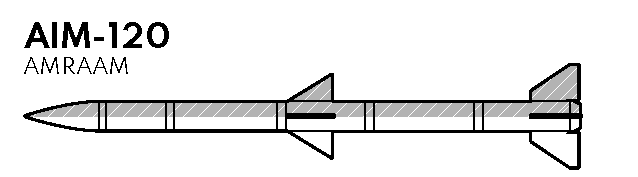
\includegraphics[
            width = 108mm,
    ]{F16_aaweapons_amraam_overview_v01.pdf}
    \caption{}
\end{figure}

\clearpage

\begin{tcoloritemize}
    \blueitem{AIM-120}{
    \begin{subitemize}
        \item \textbf{Guidance} --- Active Radar-Guided (\textbf{Fox 3})
        \item \textbf{Range} --- max:  \textasciitilde30-40nm (high mach, alt)
    \end{subitemize}}
    \blueitem{Engagement \break Types}{
    \begin{subitemize}
        \item \textbf{Single Target} --- \hyperref[subsec:aim120single]{\textbf{See \Cref{subsec:aim120single}}}
        \begin{itemize}
            \item From STT radar lock
            \item Or radar TWS / DTT tracks
        \end{itemize}
        \item \textbf{Multi Target} --- \hyperref[subsec:aim120multi]{\textbf{See \Cref{subsec:aim120multi}}}
        \begin{itemize}
            \item For TWS / DTT tracks
        \end{itemize}
    \end{subitemize}}
    \blueitem{SMS Page}{\textbf{See Figure X.XX} and below items}
    \blueitem{SLAVE / BORE}{
    \begin{subitemize}
        \item \textbf{Controls Missile Radar Line of Sight}
        \item \textbf{SLAVE}
        \begin{itemize}
            \item Missile LOS slaved to AC radar 
            \item Receives DL updates until within own radar limits
        \end{itemize}
        \item \textbf{BORE}
        \begin{itemize}
            \item Missile scans straight ahead, tracks first detected target
        \end{itemize}
    \end{subitemize}}
    \blueitem{Select AIM-120}{
    Via MFD

    \begin{subenumerate}
        \item \textbf{Selected Weapon} \dotfill \textbf{120C}
        \begin{itemize}
            \item \textbf{Cycle} --- \textbf{OSB 7} or long press \textbf{NWS}
        \end{itemize}
    \end{subenumerate}

    Via Missile Override

    \begin{subenumerate}
        \item \textbf{DGFT/MSL OVRD} \dotfill \textbf{MSL OVRD}
        \item \textbf{Selected Weapon} \dotfill Verify \textbf{120C} 
    \end{subenumerate}
    
    Via Dogfight

    \begin{subenumerate}
        \item \textbf{DGFT/MSL OVRD} \dotfill \textbf{DGFT}
        \item \textbf{Selected Weapon} \dotfill \textbf{120C}
        \begin{itemize}
            \item \textbf{Cycle} --- \textbf{OSB 7} or long press \textbf{NWS}
        \end{itemize}
    \end{subenumerate}}
    \blueitem{Selected Station}{}
\end{tcoloritemize}

\clearpage

\subsubsection{EMPLOYMENT PROFILE}

\begin{figure}[h]
    \centering
    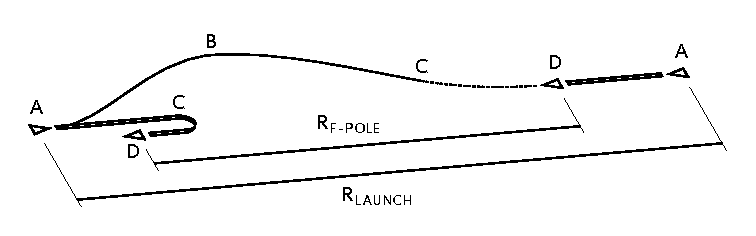
\includegraphics[
            width = 128mm,
    ]{F16_aaweapons_amraam_employment_v07.pdf}
    \caption{Generic, simplified AIM-120 employment profile}
    \label{fig:aa-weap:aim120:profile}
\end{figure}

\begin{tcoloritemize}
    \blueitem{Phases}{
    \Cref{fig:aa-weap:aim120:profile} shows AIM-120 employment profile
    including the following phases \& milestones

    \begin{subitemize}
        \item \textbf{A} --- Launch
        \item \textbf{B} --- Mid-Course Phase
        \item \textbf{C} --- Acquisition
        \item \textbf{D} --- Intercept
    \end{subitemize}}
    \blueitem{Launch}{
    \textbf{Radar Lock}

    \begin{subitemize}
        \item Only requires track to launch
        \item Target does \textbf{NOT} need to be in STT lock
    \end{subitemize}

%    \textbf{Maximizing Range --- maximizing energy}

%     \begin{subitemize}
%         \item High velocity --- increases kinetic energy
%         \item High altitude --- increases potential energy, reduces drag
%     \end{subitemize}

    \textbf{Lofting} 

    \begin{subitemize}
        \item At longer ranges the missile will loft itself to optimize trajectory
        \item Pilot can manually loft by raising the nose 20-30 deg prior to launch
    \end{subitemize}}
    \blueitem{Mid-Course Phase}{
    \textbf{Missile flies using internal IMU}

    \begin{subitemize}
        \item Receives periodic datalink updates
        \item Will fly to last updated target position if DL lost
    \end{subitemize}}
    \blueitem{Acquisition \& MPRF ``Active'' Phase}{
    Once close to DL bandit location
    \begin{subitemize}
        \item AIM-120 radar turns on in MPRF (Medium Pulse Repetition Frequency) mode 
        \item Locks on to closest / best target
    \end{subitemize}}
    \blueitem{Terminal Phase \& Intercept}{
    Once missile has gone active
    \begin{subitemize}
        \item Flies a PNG intercept trajectory towards the target locked by it's radar 
        \item Requires no further DL support, fighter can now turn away from the bandit
    \end{subitemize}}
\end{tcoloritemize}

\notebox{
    \textbf{Post-Launch Maneuvers}
    \begin{itemize}
            \item For simplicity, \cref{fig:aa-weap:aim120:profile} does not show any post-launch maneuvers until point \textbf{C}, where the missile goes active 
            % \item Depending on the tactical situation, it can be beneficial to reduce closure by turning 30-60 deg away from the bandit while maintaing radar contact 
            % \item This can be combined with a dive into thicker air to further reduce bandit missile range and maintain a look-up angle for the radar
    \end{itemize}

    \textbf{Flowing Cold}
    \begin{itemize}
        \item The fighter can turn cold prior to the missile going active
        \item Missile will fly to last DL target position, significantly reducing probability of intercept
    \end{itemize}
}

\warningbox{
    \textbf{AIM-120 HAS \underline{NO} IFF FUNCTIONALITY} --- use caution near friendlies
}

% \clearpage

\subsubsection{TACTICAL CONSIDERATIONS}

\begin{tcoloritemize}
    \blueitem{Range}{
    \textbf{Fighter-bandit distance} can be measured at different points during the timeline

    \begin{subitemize}
        \item \textbf{R\textsubscript{Launch}} --- distance at launch
        \item \textbf{R\textsubscript{F-Pole}} --- distance at impact
        \item \textbf{R\textsubscript{A-Pole}} --- distance when missile goes active
    \end{subitemize}
    
    \textbf{R\textsubscript{Launch}}, \textbf{R\textsubscript{F-Pole}} are the most relevant and should be maximized. These are visible in \cref{fig:aa-weap:aim120:profile}.
    }
    \blueitem{Maximizing Launch Range / Energy}{
    \textbf{Why?}
    \begin{subitemize}
        \item Ability to launch at longer ranges forces bandit defensive
        \item Bandit may not be able to counter-launch
        \item Higher launch energy increases P\textsubscript{intercept} %probability of intercept
    \end{subitemize}
    \textbf{How?}
    \begin{subitemize}
        \item \textbf{High velocity} --- increases kinetic energy 
        \item \textbf{High altitude} --- increases potential energy, reduces drag
    \end{subitemize}}
    \blueitem{Maximizing F-Pole Range}{
    \textbf{Why?}
    \begin{subitemize}
        \item Less likely to enter bandit launch envelope
        \item More time/range to launch 2nd missile if necessary
    \end{subitemize}
    \textbf{How?}
    \begin{subitemize}
        \item \textbf{Crank} --- turn 30-60 degrees away from bandit to reduce closure rate, maintain radar contact
        \item \textbf{Dive} --- reduces threat missile envelope
    \end{subitemize}}
    \blueitem{Flowing Cold}{
    \textbf{Why?}
    \begin{subitemize}
        \item Missile requires no support once active
        \item Defends against unknown missile launches
        \item Further maximizes F-pole range
    \end{subitemize}
    \textbf{How?}
    \begin{subitemize}
        \item \textbf{Turn} --- Away from bandit / threat
        \item \textbf{Dive} --- if necessary, reduces threat missile envelope 
    \end{subitemize}}
    \blueitem{Effect of Bandit Maneuvers}{
    As evident in \cref{fig:aa-weap:aim120:profile}, 
    R\textsubscript{Launch} is significantly greater than the distance travelled by the missile
    \begin{subitemize}
        \item DLZ calculated based off \textbf{both} own state \textbf{and} bandit state
        \begin{itemize}
            \item \textbf{Missile is relying on target to keep flying towards us}
        \end{itemize}
        \item Bandit can significantly change missile envelope by reducing closure rate / altitude
        \item If done post-launch can result in missile not having energy to intercept
    \end{subitemize}}
\end{tcoloritemize}

% \subsubsection{SYMBOLOGY}
% \begin{tcoloritemize}
%     \blueitem{HUD Symbology}{}
%     \blueitem{FCR Symbology}{}
% \end{tcoloritemize}

\marginfigeometry

\subsubsection{SINGLE TARGET EMPLOYMENT}
\label{subsec:aim120single}
\begin{checklistenumerate}
    \blueitem{Conditions}{
    \begin{subitemize}
        \item \textbf{FCR} \dotfill \textbf{ON}
        \item \textbf{RF Switch} \dotfill \textbf{NORM}
        % \item \textbf{Master Mode} \dotfill \textbf{A-A}
        \item \textbf{Selected Weapon} \dotfill \textbf{120C}
        \item \textbf{SLAVE/BORE} \dotfill Verify \textbf{SLAVE}
        \item \textbf{Master Arm} \dotfill \textbf{ARM}
    \end{subitemize}}
    \blueitem{Acquire Target}{
    \begin{subenumerate}
        \item \textbf{Target} \dotfill \textbf{Locked}
        \begin{itemize}
            \item \textbf{STT} --- from RWS, TWS, or ACM
            \item \textbf{Bug} --- from TWS
        \end{itemize}
    \end{subenumerate}}
    \blueitem{Symbology}{
    \begin{subitemize}
        \item \textbf{TLL} --- \textbf{T}arget \textbf{L}ocator \textbf{L}ine --- Extends from gun cross \& points towards target
        \item \textbf{ASEC} --- \textbf{A}llowable \textbf{S}teering \textbf{E}rror \textbf{C}ircle \\
        Changes size to reflect target state 
        \item \textbf{ASC} --- \textbf{A}ttack \textbf{S}teering \textbf{C}ue --- appears
        \item \textbf{Target Range} --- Displayed
    \end{subitemize}}
    \blueitem{Employment}{
    \begin{subenumerate}
        \item \textbf{Radar} \dotfill Locked
        \item \textbf{Maneuver} --- Place tgt within \textbf{DLZ} \& \textbf{ASEC}
        \item \textbf{WPN REL} \dotfill \textbf{Depress}
    \end{subenumerate}}
\end{checklistenumerate}

\clearpage

\subsubsection{MULTI TARGET EMPLOYMENT}
\label{subsec:aim120multi}
\begin{checklistenumerate}
    \blueitem{Conditions}{
    \begin{subitemize}
        \item \textbf{FCR} \dotfill \textbf{ON}
        \item \textbf{RF Switch} \dotfill \textbf{NORM}
        % \item \textbf{Master Mode} \dotfill \textbf{A-A}
        \item \textbf{Selected Weapon} \dotfill \textbf{120C}
        \item \textbf{SLAVE/BORE} \dotfill Verify \textbf{SLAVE}
        \item \textbf{Master Arm} \dotfill \textbf{ARM}
    \end{subitemize}}
    \blueitem{Acquire Targets}{From RWS/DTT or TWS

    \begin{subenumerate}
        \item \textbf{Targets} \dotfill Designate with \textbf{TMS Fwd}
        \begin{itemize}
            \item \textbf{TWS} --- Repeat for all desired targets 
            \item \textbf{DTT} --- Repeat for second target
        \end{itemize}
    \end{subenumerate}}
    \blueitem{Symbology}{
    \begin{subitemize}
        \item \textbf{TLL} --- \textbf{T}arget \textbf{L}ocator \textbf{L}ine --- Extends from gun cross \& points towards target
        \item \textbf{ASEC} --- \textbf{A}llowable \textbf{S}teering \textbf{E}rror \textbf{C}ircle \\
        Changes size to reflect target state 
        \item \textbf{ASC} --- \textbf{A}ttack \textbf{S}teering \textbf{C}ue --- appears
        \item \textbf{Target Range} --- Displayed
    \end{subitemize}}
    \blueitem{Employment}{
    \begin{subenumerate}
        \item \textbf{Desired Targets} \dotfill Tracked
        \item \label{item:aim120:multitgt:steer}\textbf{Current Target} --- Place within \textbf{DLZ} \& \textbf{ASEC}
        \item \label{item:aim120:multitgt:fire}\textbf{WPN REL} \dotfill \textbf{Depress}
        \item \label{item:aim120:multitgt:cycle}\textbf{Target} \dotfill Cycle with \textbf{TMS Right} 
    \end{subenumerate}

    Repeat \ref{item:aim120:multitgt:steer}-\ref{item:aim120:multitgt:cycle} for all remaining targets}
\end{checklistenumerate}

\notebox{
    \begin{itemize}
        \item \textbf{Single Target TWS Employment} --- special case of multi-target
    \end{itemize}
}

\marginfigrestore